\documentclass[10pt,twoside]{article}
\newcommand{\reporttitle}{ARM LAB}
\newcommand{\reportauthors}{Tiger Cross, William Burr, Matt Malarkey, Daniel Hails}
\newcommand{\reporttype}{Interim Report}

% include files that load packages and define macros
\usepackage{wrapfig}
%%%%%%%%%%%%%%%%%%%%%%%%%%%%%%%%%%%%%%%%%
% University Assignment Title Page 
% LaTeX Template
% Version 1.0 (27/12/12)
%
% This template has been downloaded from:
% http://www.LaTeXTemplates.com
%
% Original author:
% WikiBooks (http://en.wikibooks.org/wiki/LaTeX/Title_Creation)
%
% License:
% CC BY-NC-SA 3.0 (http://creativecommons.org/licenses/by-nc-sa/3.0/)
% 
% Instructions for using this template:
% This title page is capable of being compiled as is. This is not useful for 
% including it in another document. To do this, you have two options: 
%
% 1) Copy/paste everything between \begin{document} and \end{document} 
% starting at \begin{titlepage} and paste this into another LaTeX file where you 
% want your title page.
% OR
% 2) Remove everything outside the \begin{titlepage} and \end{titlepage} and 
% move this file to the same directory as the LaTeX file you wish to add it to. 
% Then add \input{./title_page_1.tex} to your LaTeX file where you want your
% title page.
%
%----------------------------------------------------------------------------------------
%	PACKAGES AND OTHER DOCUMENT CONFIGURATIONS
%----------------------------------------------------------------------------------------
\usepackage{ifxetex}
\usepackage{textpos}
\usepackage{natbib}
\usepackage{kpfonts}
\usepackage[a4paper,hmargin=2.8cm,vmargin=2.0cm,includeheadfoot]{geometry}
\usepackage{ifxetex}
\usepackage{stackengine}
\usepackage{tabularx,longtable,multirow,subfigure,caption}%hangcaption
\usepackage{fncylab} %formatting of labels
\usepackage{fancyhdr}
\usepackage{color}
\usepackage[tight,ugly]{units}
\usepackage{url}
\usepackage{float}
\usepackage[english]{babel}
\usepackage{amsmath}
\usepackage{graphicx}
\usepackage[colorinlistoftodos]{todonotes}
\usepackage{dsfont}
\usepackage{epstopdf} % automatically replace .eps with .pdf in graphics
\usepackage{natbib}
\usepackage{backref}
\usepackage{array}
\usepackage{latexsym}
\usepackage{etoolbox}

\usepackage{enumerate} % for numbering with [a)] format 



\ifxetex
\usepackage{fontspec}
\setmainfont[Scale=.8]{OpenDyslexic-Regular}
\else
\usepackage[pdftex,pagebackref,hypertexnames=false,colorlinks]{hyperref} % provide links in pdf
\hypersetup{pdftitle={},
  pdfsubject={}, 
  pdfauthor={\reportauthors},
  pdfkeywords={}, 
  pdfstartview=FitH,
  pdfpagemode={UseOutlines},% None, FullScreen, UseOutlines
  bookmarksnumbered=true, bookmarksopen=true, colorlinks,
    citecolor=black,%
    filecolor=black,%
    linkcolor=black,%
    urlcolor=black}
\usepackage[all]{hypcap}
\fi

\usepackage{tcolorbox}

% various theorems
\usepackage{ntheorem}
\theoremstyle{break}
\newtheorem{lemma}{Lemma}
\newtheorem{theorem}{Theorem}
\newtheorem{remark}{Remark}
\newtheorem{definition}{Definition}
\newtheorem{proof}{Proof}

% example-environment
\newenvironment{example}[1][]
{ 
\vspace{4mm}
\noindent\makebox[\linewidth]{\rule{\hsize}{1.5pt}}
\textbf{Example #1}\\
}
{ 
\noindent\newline\makebox[\linewidth]{\rule{\hsize}{1.0pt}}
}



%\renewcommand{\rmdefault}{pplx} % Palatino
% \renewcommand{\rmdefault}{put} % Utopia

\ifxetex
\else
\renewcommand*{\rmdefault}{bch} % Charter
\renewcommand*{\ttdefault}{cmtt} % Computer Modern Typewriter
%\renewcommand*{\rmdefault}{phv} % Helvetica
%\renewcommand*{\rmdefault}{iwona} % Avant Garde
\fi

\setlength{\parindent}{0em}  % indentation of paragraph

\setlength{\headheight}{14.5pt}
\pagestyle{fancy}
\fancyfoot[ER,OL]{\thepage}%Page no. in the left on
                                %odd pages and on right on even pages
\fancyfoot[OC,EC]{\sffamily }
\renewcommand{\headrulewidth}{0.1pt}
\renewcommand{\footrulewidth}{0.1pt}
\captionsetup{margin=10pt,font=small,labelfont=bf}


%--- chapter heading

\def\@makechapterhead#1{%
  \vspace*{10\p@}%
  {\parindent \z@ \raggedright %\sffamily
        %{\Large \MakeUppercase{\@chapapp} \space \thechapter}
        %\\
        %\hrulefill
        %\par\nobreak
        %\vskip 10\p@
    \interlinepenalty\@M
    \Huge \bfseries 
    \thechapter \space\space #1\par\nobreak
    \vskip 30\p@
  }}

%---chapter heading for \chapter*  
\def\@makeschapterhead#1{%
  \vspace*{10\p@}%
  {\parindent \z@ \raggedright
    \sffamily
    \interlinepenalty\@M
    \Huge \bfseries  
    #1\par\nobreak
    \vskip 30\p@
  }}
  



% %%%%%%%%%%%%% boxit
\def\Beginboxit
   {\par
    \vbox\bgroup
	   \hrule
	   \hbox\bgroup
		  \vrule \kern1.2pt %
		  \vbox\bgroup\kern1.2pt
   }

\def\Endboxit{%
			      \kern1.2pt
		       \egroup
		  \kern1.2pt\vrule
		\egroup
	   \hrule
	 \egroup
   }	

\newenvironment{boxit}{\Beginboxit}{\Endboxit}
\newenvironment{boxit*}{\Beginboxit\hbox to\hsize{}}{\Endboxit}



\allowdisplaybreaks

\makeatletter
\newcounter{elimination@steps}
\newcolumntype{R}[1]{>{\raggedleft\arraybackslash$}p{#1}<{$}}
\def\elimination@num@rights{}
\def\elimination@num@variables{}
\def\elimination@col@width{}
\newenvironment{elimination}[4][0]
{
    \setcounter{elimination@steps}{0}
    \def\elimination@num@rights{#1}
    \def\elimination@num@variables{#2}
    \def\elimination@col@width{#3}
    \renewcommand{\arraystretch}{#4}
    \start@align\@ne\st@rredtrue\m@ne
}
{
    \endalign
    \ignorespacesafterend
}
\newcommand{\eliminationstep}[2]
{
    \ifnum\value{elimination@steps}>0\leadsto\quad\fi
    \left[
        \ifnum\elimination@num@rights>0
            \begin{array}
            {@{}*{\elimination@num@variables}{R{\elimination@col@width}}
            |@{}*{\elimination@num@rights}{R{\elimination@col@width}}}
        \else
            \begin{array}
            {@{}*{\elimination@num@variables}{R{\elimination@col@width}}}
        \fi
            #1
        \end{array}
    \right]
    & 
    \begin{array}{l}
        #2
    \end{array}
    &%                                    moved second & here
    \addtocounter{elimination@steps}{1}
}
\makeatother

%% Fast macro for column vectors
\makeatletter  
\def\colvec#1{\expandafter\colvec@i#1,,,,,,,,,\@nil}
\def\colvec@i#1,#2,#3,#4,#5,#6,#7,#8,#9\@nil{% 
  \ifx$#2$ \begin{bmatrix}#1\end{bmatrix} \else
    \ifx$#3$ \begin{bmatrix}#1\\#2\end{bmatrix} \else
      \ifx$#4$ \begin{bmatrix}#1\\#2\\#3\end{bmatrix}\else
        \ifx$#5$ \begin{bmatrix}#1\\#2\\#3\\#4\end{bmatrix}\else
          \ifx$#6$ \begin{bmatrix}#1\\#2\\#3\\#4\\#5\end{bmatrix}\else
            \ifx$#7$ \begin{bmatrix}#1\\#2\\#3\\#4\\#5\\#6\end{bmatrix}\else
              \ifx$#8$ \begin{bmatrix}#1\\#2\\#3\\#4\\#5\\#6\\#7\end{bmatrix}\else
                 \PackageError{Column Vector}{The vector you tried to write is too big, use bmatrix instead}{Try using the bmatrix environment}
              \fi
            \fi
          \fi
        \fi
      \fi
    \fi
  \fi 
}  
\makeatother

\robustify{\colvec}

%%% Local Variables: 
%%% mode: latex
%%% TeX-master: "notes"
%%% End: 

% quick way of adding a figure
\newcommand{\fig}[3]{
 \begin{center}
 \scalebox{#3}{\includegraphics[#2]{#1}}
 \end{center}
}

%\newcommand*{\point}[1]{\vec{\mkern0mu#1}}
\newcommand{\ci}[0]{\perp\!\!\!\!\!\perp} % conditional independence
\newcommand{\point}[1]{{#1}} % points 
\renewcommand{\vec}[1]{{\boldsymbol{{#1}}}} % vector
\newcommand{\mat}[1]{{\boldsymbol{{#1}}}} % matrix
\newcommand{\R}[0]{\mathds{R}} % real numbers
\newcommand{\Z}[0]{\mathds{Z}} % integers
\newcommand{\N}[0]{\mathds{N}} % natural numbers
\newcommand{\nat}[0]{\mathds{N}} % natural numbers
\newcommand{\Q}[0]{\mathds{Q}} % rational numbers
\ifxetex
\newcommand{\C}[0]{\mathds{C}} % complex numbers
\else
\newcommand{\C}[0]{\mathds{C}} % complex numbers
\fi
\newcommand{\tr}[0]{\text{tr}} % trace
\renewcommand{\d}[0]{\mathrm{d}} % total derivative
\newcommand{\inv}{^{-1}} % inverse
\newcommand{\id}{\mathrm{id}} % identity mapping
\renewcommand{\dim}{\mathrm{dim}} % dimension
\newcommand{\rank}[0]{\mathrm{rk}} % rank
\newcommand{\determ}[1]{\mathrm{det}(#1)} % determinant
\newcommand{\scp}[2]{\langle #1 , #2 \rangle}
\newcommand{\kernel}[0]{\mathrm{ker}} % kernel/nullspace
\newcommand{\img}[0]{\mathrm{Im}} % image
\newcommand{\idx}[1]{{(#1)}}
\DeclareMathOperator*{\diag}{diag}
\newcommand{\E}{\mathds{E}} % expectation
\newcommand{\var}{\mathds{V}} % variance
\newcommand{\gauss}[2]{\mathcal{N}\big(#1,\,#2\big)} % gaussian distribution N(.,.)
\newcommand{\gaussx}[3]{\mathcal{N}\big(#1\,|\,#2,\,#3\big)} % gaussian distribution N(.|.,.)
\newcommand{\gaussBig}[2]{\mathcal{N}\left(#1,\,#2\right)} % see above, but with brackets that adjust to the height of the arguments
\newcommand{\gaussxBig}[3]{\mathcal{N}\left(#1\,|\,#2,\,#3\right)} % see above, but with brackets that adjust to the height of the arguments
\DeclareMathOperator{\cov}{Cov} % covariance (matrix) 
\ifxetex
\renewcommand{\T}[0]{^\top} % transpose
\else
\newcommand{\T}[0]{^\top}
\fi
% matrix determinant
\newcommand{\matdet}[1]{
\left|
\begin{matrix}
#1
\end{matrix}
\right|
}



%%% various color definitions
\definecolor{darkgreen}{rgb}{0,0.6,0}

\newcommand{\blue}[1]{{\color{blue}#1}}
\newcommand{\red}[1]{{\color{red}#1}}
\newcommand{\green}[1]{{\color{darkgreen}#1}}
\newcommand{\orange}[1]{{\color{orange}#1}}
\newcommand{\magenta}[1]{{\color{magenta}#1}}
\newcommand{\cyan}[1]{{\color{cyan}#1}}


% redefine emph
\renewcommand{\emph}[1]{\blue{\bf{#1}}}

% place a colored box around a character
\gdef\colchar#1#2{%
  \tikz[baseline]{%
  \node[anchor=base,inner sep=2pt,outer sep=0pt,fill = #2!20] {#1};
    }%
}%
 % short-hand notation and macros

%%%%%%%%%%%%%%%%%%%%%%%%%%%%

\begin{document}
% front page

%%%%%%%%%%%%%%%%%%%%%%%%%%%% Main document
\begin{center}
\LARGE\textbf{ARM Checkpoint Report}
\end{center}
\begin{center}
\small{Tiger Cross, William Burr, Matt Malarkey, Daniel Hails - 1st June 2018}
\end{center}

\section{Code Structure}
\subsection*{Files}
We decided to employ a divide and conquer approach to building the emulator, splitting the problem into smaller sub-problems each with their own file. This allowed for a modular structure where functions, and definitions are reusable:
\begin{itemize}
\item \textbf{arm.h} - Contains definitions/typedefs for program state, registers, pipeline, flags, conditions and opcodes.
\item \textbf{instructions.h} - Contains typedefs for representing decoded binary instructions. See Figure 1.
\item \textbf{emulate.c (.h)} - This is entry for the emulator and contains the main function which initialises memory and registers, loops through binary instructions, decoding and executing each using the pipeline until reaching halt. 
\item \textbf{decode.c (.h)} - Takes in a binary instruction (a word) and returns an instance of an instruction struct (instruction\_t in \textbf{instructions.h}) representing the decoded binary.
\item \textbf{execute.c (.h)} - Takes in program state, and executes the decoded instruction\_t in pipeline, modifying the state (registers and memory) based on the instruction.
\item \textbf{io.c (.h)} - Contains functions for getting/setting words in memory, printing register and memory contents, reading and writing to/from files. 
\item \textbf{bitops.c (.h)} - Contains functions for extracting bits from a word, left and right shifts, arithmetic and logical rotations, negating words, checking if words are negative and left padding with 0s.
\item \textbf{register.c (.h)} - Contains functions for getting/setting registers, getting/setting PC, incrementing PC, getting/setting flags (from CPSR).
\item \textbf{error.c (.h)} - Contains typedefs for error codes, error strings and functions for printing errors and dealing with error codes.
\end{itemize}
\begin{wrapfigure}[11]{R}{0.5\textwidth}
\centering
\vspace{-20pt}
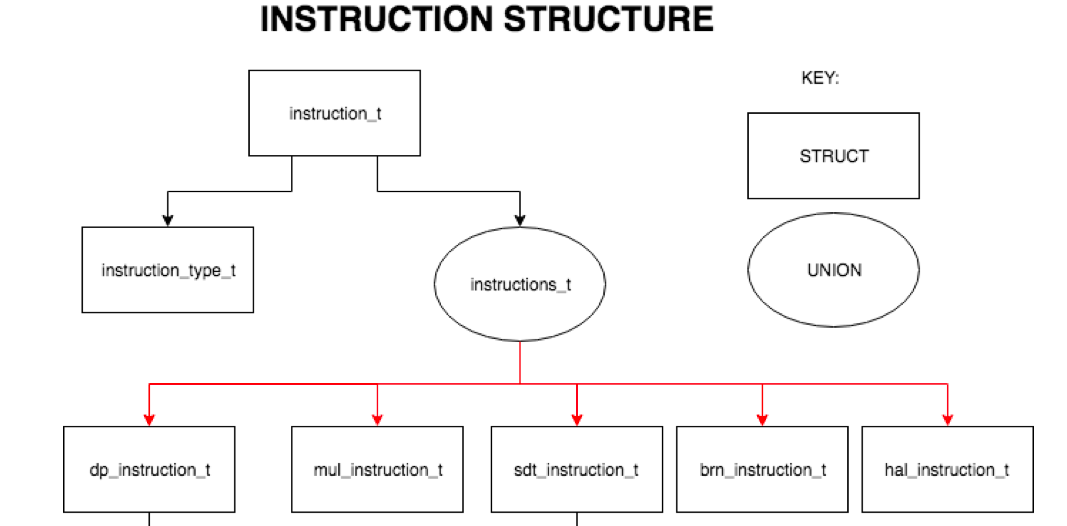
\includegraphics[width=\hsize]{figures/ARMStructure}
\caption{\label{fig:ARMStructure} Extract of struct/union hierarchy for instruction\_t in \textbf{instructions.h}}.
\end{wrapfigure}

Unit tests were used to identify and resolve errors in each module, before combining modules together to form the emulator. \\ 
To provide clarity in team about how we were to decode instructions, a diagram was constructed illustrating the hierarchy of unions and structs in \textbf{instructions.h}. \\ 
An extract of this diagram is shown in Figure 1, with the full version in the git docs repository which includes additional structs and unions for the offset/operand for the SDT and DP instructions respectively. 
\subsection*{Reusable Components}
For the assembler, elements of the existing code will prove useful. These elements include \textbf{instructions.h} as each ARM instruction can be translated into a respective instruction\_t, then translated to binary. \textbf{io.c (.h)} will be useful for reading in the instructions from a file and writing the binary to another file. \textbf{bitops.c (.h)} will be useful for applying shifts to binary words in the construction of the assembled binary instruction. 

\section{Group Work}
\subsection*{Planning and Delegation}
\begin{wrapfigure}[10]{R}{0.55\textwidth}
\centering
\vspace{-40pt}
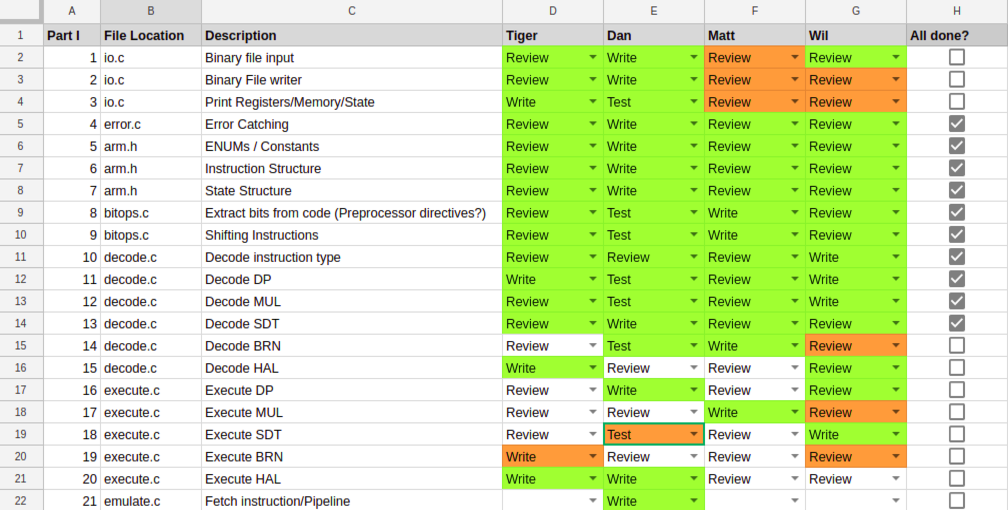
\includegraphics[width=0.6\textwidth]{figures/WorkloadBreakdown.png}
\caption{\label{fig:spreadsheet} Spreadsheet to show our allocation of tasks.}
\end{wrapfigure}
In our first meeting we broke down part I into small tasks and created a spreadsheet to assign tasks to members based on their preferences and strengths. We opted for a colour-coded system for illustrating the progress of tasks. A copy of the table midway through part I is shown in Figure 2. Despite initial assignments, each group members was available to help and assist with any task.

\subsection*{Communication and Use of Git}
\begin{wrapfigure}[13]{L}{0.4\textwidth}
\centering
\vspace{-16pt}
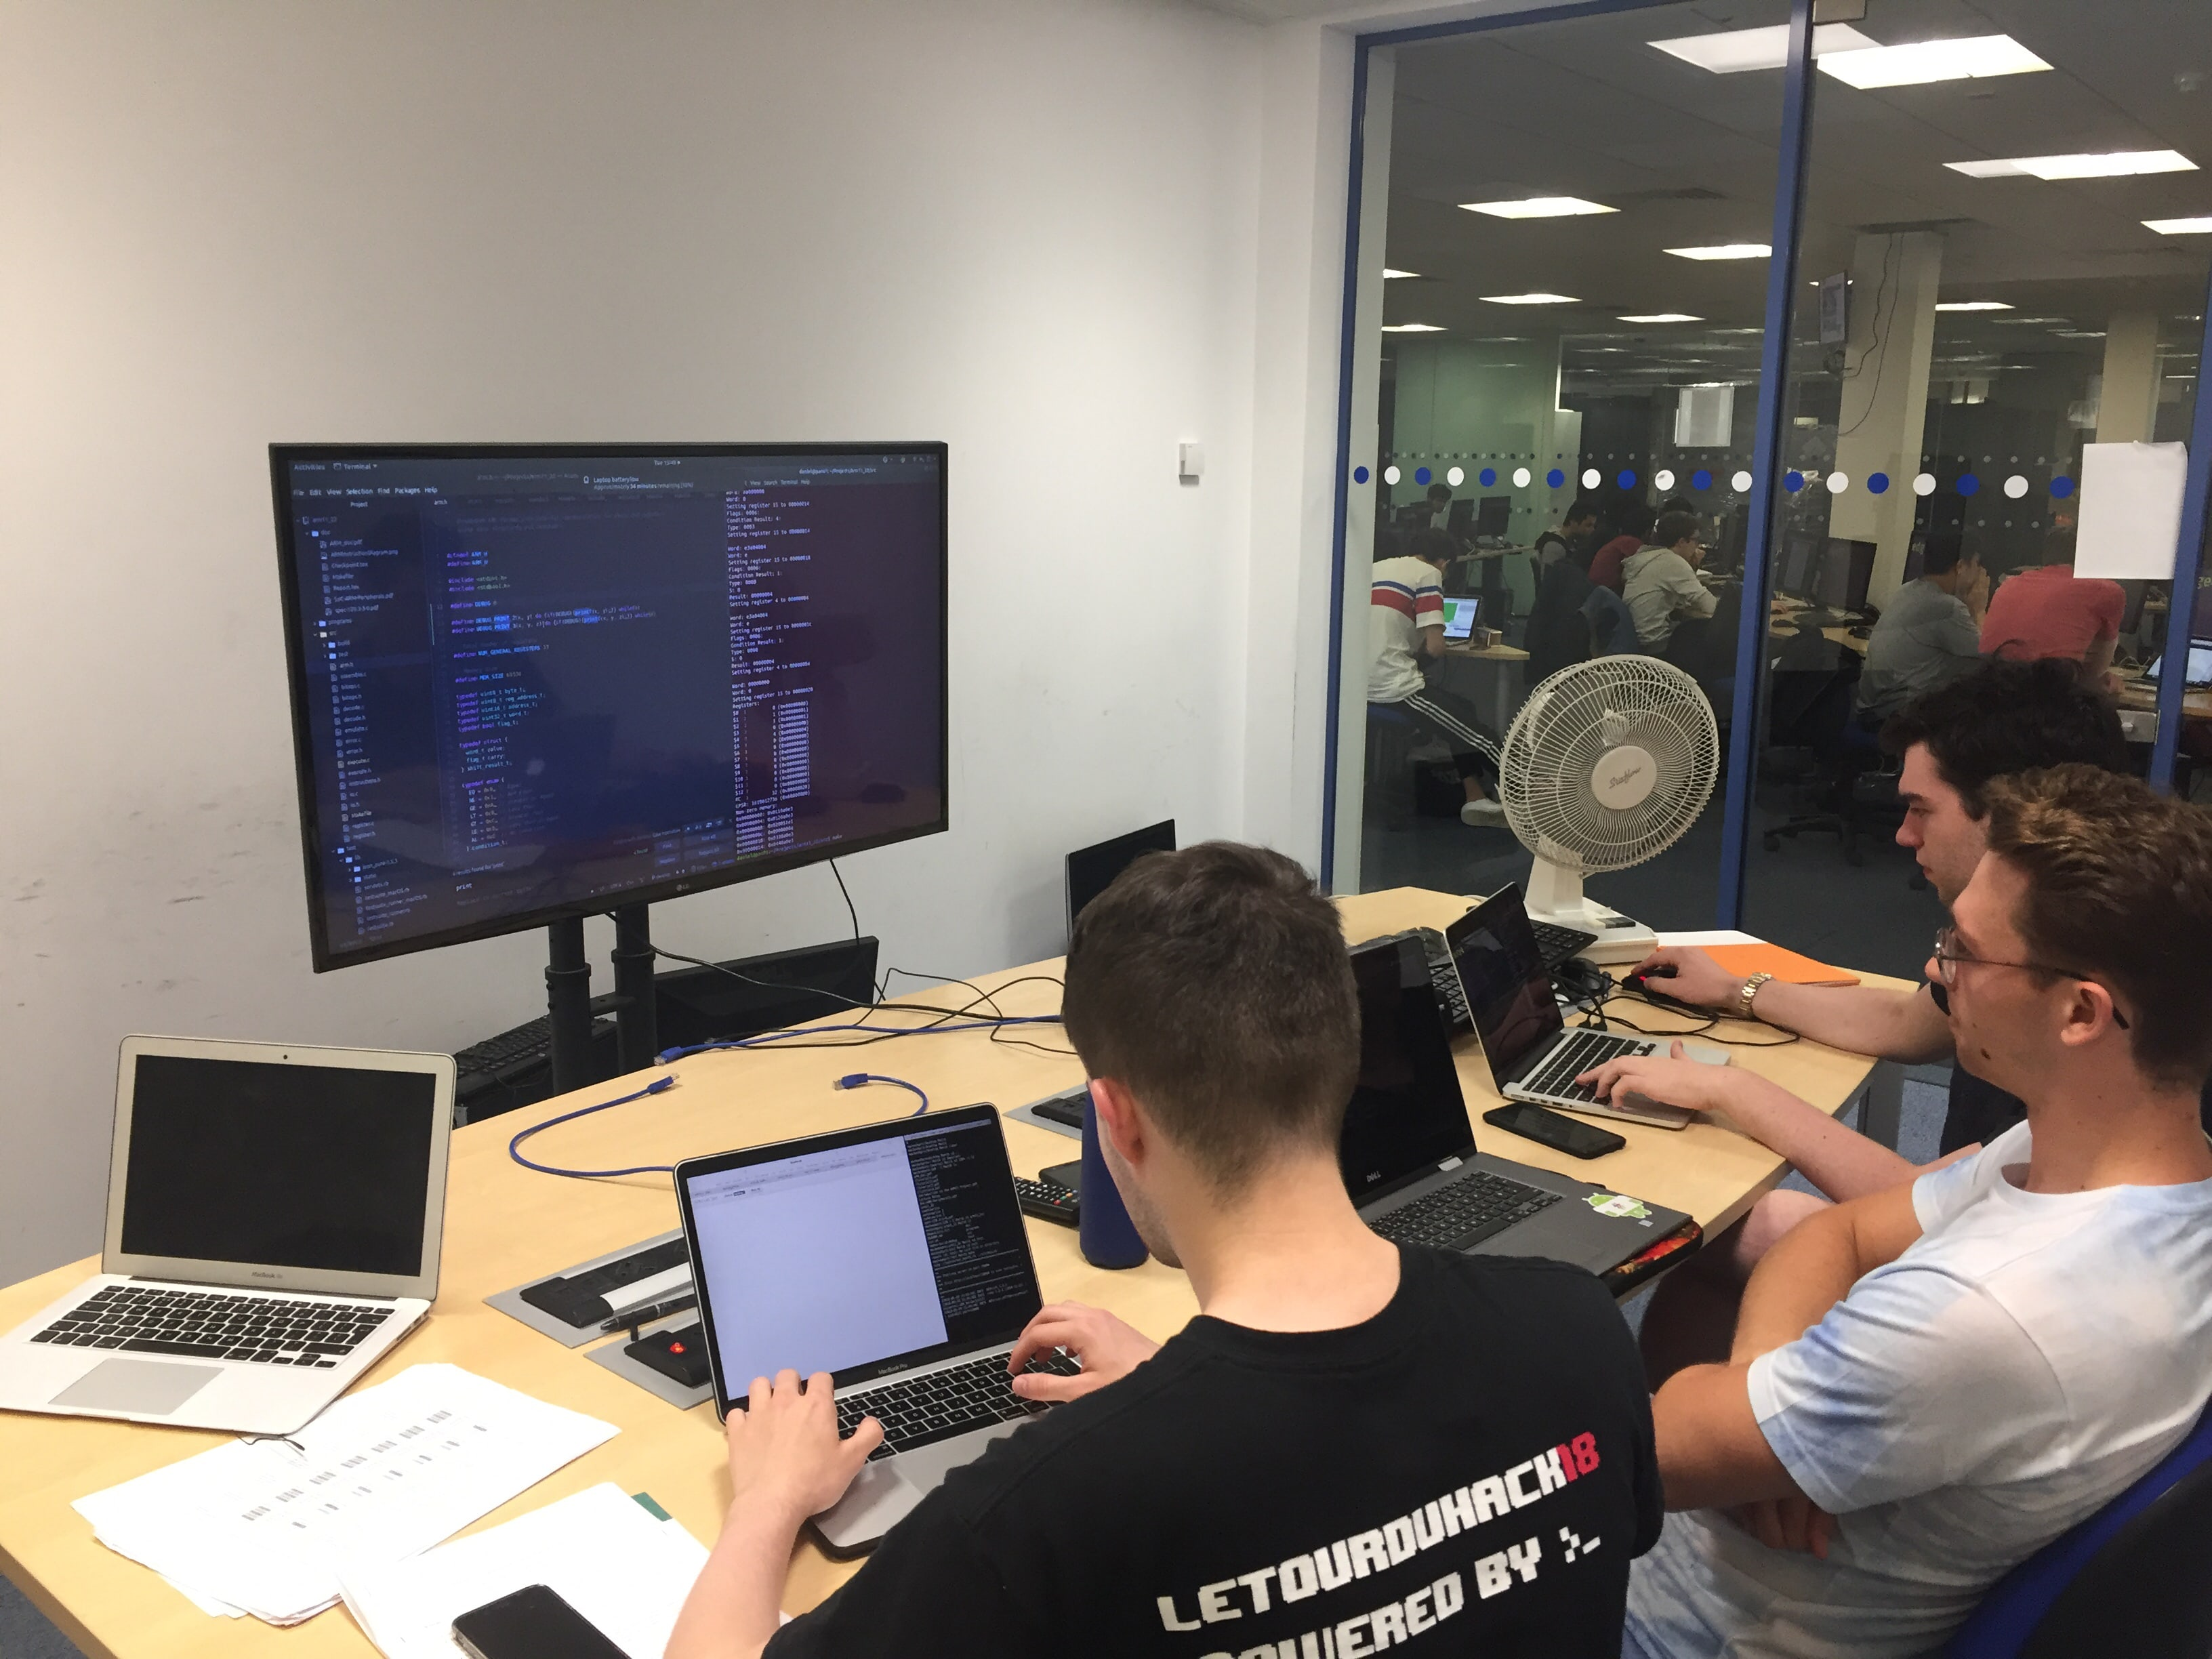
\includegraphics[width=0.4\textwidth]{figures/Group_debug_sesh-min.jpg}
\caption{\label{fig:spreadsheet} Group Debug Session in Huxley}
\end{wrapfigure}
Throughout the project so far we have favoured face-to-face communication over other methods, especially whilst debugging (a group debug session is shown in Figure 3) as we can communicate clearly with one another. Outside of college, we initially used Facebook messenger but found we needed clearer communication. We therefore created our own Slack workspace, creating channels for each module in development. This allowed us to discuss multiple areas clearly and help each other with problems on specific channels.\\
\linebreak

For using Gitlab, we created a \textbf{develop} branch which would contain a working version of our emulator/assembler with the goal of pushing to \textbf{master} when we are confident that it is production level. For each task, we created branches from \textbf{develop} (e.g. \textbf{decodeBRN}, \textbf{decodeMul} etc.), but then decided to reduce unnecessary branching by only creating new branches from \textbf{develop} for each module (e.g. \textbf{execute}, \textbf{bitops}, \textbf{error}). For each branch, when the module/task was finished the team member would submit a merge request, prompting another member to review the changes and approve the merge. This ensured we developed and reviewed code as a team in a structured way.

\section{Future Challenges}

For each challenge in the upcoming parts, we have designed our approach accordingly:
\begin{itemize}

\item \textbf{Part II} - To ensure the on-time development of a working, well-structured assembler, we have decided the structure as a team and have split the assembler into modules, each with its own assigned team members, slack channel and git branch. Team deadline: 9:00am, 4th June.
\item \textbf{Part III} - Since this is a small task, we have already set about producing the ARM code for repeatedly switching the LED on and off, and have successfully tested this using an online ARM compiler. The only remaining task is to modify Part I to accommodate the changes. 
\item \textbf{Extension} - We anticipate this section to be very time consuming, so we already have an active slack channel, \textbf{\#extension}, for brainstorming and planning ideas, including finding any necessary parts we may need to order early. This will allow us to be ready with a plan and with the right hardware by the time the other parts are done. \\
Since there will be no given specification, we will be constructing our own specification of what our extension will do, so that the team has a clear understanding of the design.
\end{itemize}

\end{document}
%%% Local Variables: 
%%% mode: latex
%%% TeX-master: t
%%% End: 
